\chapter{\IfLanguageName{dutch}{Stand van zaken}{State of the art}}%
\label{ch:stand-van-zaken}

% Tip: Begin elk hoofdstuk met een paragraaf inleiding die beschrijft hoe
% dit hoofdstuk past binnen het geheel van de bachelorproef. Geef in het
% bijzonder aan wat de link is met het vorige en volgende hoofdstuk.

% Pas na deze inleidende paragraaf komt de eerste sectiehoofding.
In de digitale wereld van vandaag is data de sleutel tot succes. Bedrijven verzamelen en analyseren data om hun klanten beter te begrijpen, hun marketingstrategieën te optimaliseren, en hun concurrentiepositie te versterken \autocite{OnesiOzigagun2024},
Deze enorme vraag naar kwalitatieve data drijft de ontwikkeling van nieuwe en innovatieve methodes voor dataverzameling. Er zijn vele manieren waarop er aan dataverzameling kan gedaan worden, deze studie focust zich op web scraping.

\section{Webscraping}
Webscraping is een techniek die via scripting data extraheert van websites~\autocite{Khder2021}. Deze data kan in verschillende formaten voorkomen, zoals HTML, JSON, XML en CSV. Webscraping heeft tal van toepassingen, waaronder:
\begin{itemize}
    \item Data-extractie, dit is het verzamelen van data van websites voor diverse doeleinden,
    zoals marktonderzoek,prijsvergelijking en het verzamelen van recensies
    \item Het automatiseren van taken die anders handmatig zouden moeten worden uitgevoerd, denk maar
    aan het invullen van bepaalde formulieren, aanmaken van documenten en downloaden van bestanden
    \item Monitoren van websites voor veranderingen van prijzen, nieuwe producten of statussen van bepaalde zaken
\end{itemize}


\subsection{Traditionele web scraping}
In dit hoofdstuk wordt traditionele webscraping  onderzocht als een techniek voor het extraheren van data van websites door het parsen van de HTML-code van websites. De focus ligt op het begrijpen van de werking van traditionele webscraping, het identificeren van de voor- en nadelen ervan, en het verkennen van enkele alternatieve methoden.
~
Traditionele webscraping begint met het identificeren van de doelpagina die de gewenste data bevat. Vervolgens wordt de HTML-code van de doelpagina opgehaald via een HTTP-request. Deze stap kan worden uitgevoerd met de developer tools  in de browser, Postman of met een van de meest gebruikte Python-bibliotheken requests \autocite{Nate2023}.  Na het verkrijgen van de HTML-code wordt deze geparset om er de gewenste gegevens uit te halen. Dit kan gedaan worden met de Python-bibliotheek BeautifulSoup. De verkregen data kan daarna worden omgezet in verschillende data formaten zoals JSON, CSV en XML of het kan rechtstreeks  in een database of een ander bestandssysteem gestoken worden.
\begin{figure}[h]
    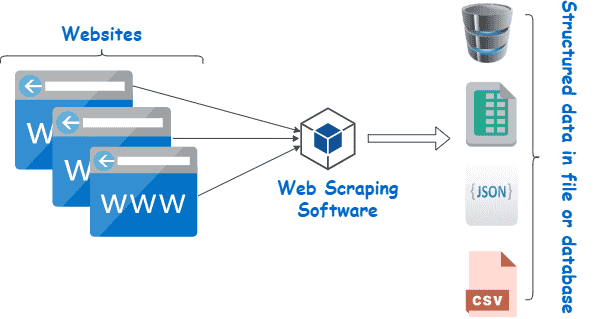
\includegraphics[width=\linewidth]{graphics/webscraping2.png}
    \caption{De werking van een web scraper \autocite{Kinsta2022}}
    \label{fig:webscraping}
\end{figure}

Enkele voordelen van de traditionele webscraping manier zijn:
\begin{itemize}
    \item \textbf{Eenvoudig}: Traditionele webscraping is een van de eenvoudigere methodes die met weinig technische kennis kan worden toegepast. Deze zijn eenvoudig in de zin dat je met zeer weinig code al een basis scraper kan bouwen. In codefragment \ref{code:example1} is een voorbeeld te zien van een eenvoudige traditionele webscraper, geschreven in de programmeertaal Python. Deze webscraper geeft de titel weer van de website die men wenst te scrapen.

    \begin{lstlisting}[language=python, captionpos=b, caption={Een voorbeeld van een eenvoudige webscraper.}, label={code:example1}]
        # Importeer de nodige Python-bibliotheek
        import requests
        from bs4 import BeautifulSoup

        # De url die gescraped zal worden
        url = "https://webscraper.io/test-sites/e-commerce/static"

        # De inhoud van de url ophalen
        page = requests.get(url)

        # Controle of het gelukt is om de inhoud op te halen
        if page.ok:

            # Parsen van de inhoud
            soup = BeautifulSoup(page.content, 'html.parser')

            # Opzoeken van de titel van de opgehaalde url
            title = soup.find("title")
            result = title.get_text()

            print(title)
    \end{lstlisting}

    \item \textbf{Repliceerbaarheid}: De manier waarop de website wordt binnengehaald in deze traditionele webscrapers is voor iedere website hetzelfde, namelijk het ophalen van de HTML-code van de website . Dit zorgt ervoor dat deze scrapers makkelijk te hergebruiken zijn.
\end{itemize}

Deze eenvoud komt echter niet zonder kost, hier zijn de nadelen van traditionele webscrapers:

\begin{itemize}
    \item \textbf{Beperkte functionaliteit: }De oorspronkelijke en eerste webscrapingmethoden zijn beperkt tot het extraheren van gegevens die expliciet zijn opgenomen in de HTML-code van de website, waardoor ze niet in staat zijn om data te verzamelen die via dynamische scripts, zoals JavaScript, worden geladen of die zich achter interactieve elementen bevinden.

    \item \textbf{Onderhoud}: Websites en dus ook hun HTML-code veranderen voortdurend, waardoor webscraping scripts regelmatig moeten worden bijgewerkt zodat ze hun correcte werking behouden.

    \item \textbf{Parsen}: Wanneer de HTML-structuur complex en/of niet consistent is, kan dit aanzienlijke problemen veroorzaken bij het parsen van HTML-code. Een inconsistente HTML-structuur zorgt ervoor dat de gezochte data mogelijk niet in dezelfde tag staat als op een vorige pagina van dezelfde website. Dit betekent dat dezelfde informatie op verschillende pagina's in verschillende HTML-elementen kan staan. Daarnaast kan de tag waarin de data is geplaatst, zich onder verschillende parent-tags bevinden. Deze variabiliteit compliceert het proces van gegevensextractie en vereist vaak extra inspanning en geavanceerde methoden om nauwkeurig en efficiënt data te kunnen verzamelen.
    De volgende twee code fragmenten~\ref{code:HTML1}  en~\ref{code:HTML2} maken gebruik van verschillende HTML-tags en andere klasse namen. Toch geven deze twee code fragmenten hetzelfde resultaat zoals in figuur \ref{fig:inconsistente HTML}  te zien is.

    \begin{figure}[h]
        \centering
        
\includegraphics{graphics/HTML-voorbeeld.png}
        \caption{Het resultaat van code fragmenten~\ref{code:HTML1} en~\ref{code:HTML2}}
        \label{fig:inconsistente HTML}
    \end{figure}

    \begin{listing}
        \begin{lstlisting}[language=HTML, caption={HTML voorbeeld 1},label={code:HTML1}]
            <body>
                <div class="product">
                    <h3 class="product-naam">Product A</h3>
                    <span class="prijs">€10</span>
                    <p class="description">Beschrijving Product A</p>
                </div>
            </body>
        \end{lstlisting}

        \begin{lstlisting}[language=HTML,caption={HTML voorbeeld 2},label={code:HTML2}]
            <body>
                <div class="product">
                    <h3 class="naam">Product A</h3>
                    <span class="product-prijs">€10</span>
                    <p class="product-description">Beschrijving Product A</p>
                </div>
            </body>
        \end{lstlisting}
    \end{listing}

    \item \textbf{Efficiëntie}: De traditionele webscraping methode haalt de volledige webpagina binnen. Dit wil zeggen dat voor een webscraper die de prijs van één artikel ophaalt, de volledige webpagina wordt geëxtraheerd. Bij grote websites met veel webpagina's zorgt dit op 2 plaatsen voor vertraging. Eerst moet deze volledige webpagina opgehaald worden, daarna wordt deze geparset en dan pas dan kan men op zoek naar de data.
\end{itemize}

Een alternatieve manier om aan webscraping te doen is aan de hand van API's. Websites bieden soms API's (Application Programming Interfaces) aan die het mogelijk maken om data te verzamelen in een gestructureerd formaat~\autocite{Ayushi2021}. API's zijn ontworpen voor developers en bieden een gestandaardiseerde manier om data te communiceren.

\subsection{API webscraping}

Een van de belangrijkste voordelen van API's is hun gebruiksgemak. Ze bieden een gestandaardiseerde interface waarmee gebruikers eenvoudig toegang kunnen krijgen tot de gewenste gegevens. Dit maakt het proces van gegevensverzameling efficiënter en toegankelijker, zelfs voor gebruikers met beperkte technische vaardigheden. Bovendien worden API's over het algemeen onderhouden door de website-eigenaar, wat de betrouwbaarheid van de gegevensstroom verhoogt in vergelijking met webscraping, waarbij de structuur van de website kan veranderen zonder voorafgaande kennisgeving, wat leidt tot inconsistenties in de gegevens. Een ander voordeel van API's is hun snelheid. In vergelijking met webscraping kunnen API's gegevens sneller leveren doordat ze directe toegang hebben tot de backend van de website, waardoor de latentie wordt verminderd en de totale efficiëntie van het verzamelproces wordt verbeterd.
\vspace{5mm} %5mm vertical space

Ondanks deze voordelen zijn er echter ook nadelen verbonden aan het gebruik van API's. Een van de belangrijkste beperkingen is de beschikbaarheid ervan. Niet alle websites bieden API's aan, dit limiteert de mogelijkheden voor gegevensverzameling , vooral bij het werken met minder bekende bronnen.
Daarnaast kunnen API's beperkte functionaliteit bieden, waarbij mogelijk niet alle benodigde gegevens beschikbaar zijn via de API. Dit kan gebruikers dwingen om toch andere methoden te gebruiken om aanvullende gegevens te verkrijgen, wat de complexiteit van het verzamelproces kan vergroten.
Een ander nadeel van het gebruik van API's is het vereiste authenticatieproces. Sommige API's vereisen dat gebruikers zich authentiseren alvorens ze toegang krijgen tot de API, wat extra stappen met zich meebrengt en de implementatie kan compliceren.

\subsection{Netwerkverkeersanalyse}
Netwerkverkeersanalyse, ook bekend als packet sniffing of network sniffing, is een techniek waarbij gegevenspakketten die over een netwerk worden verzonden, worden onderschept en geanalyseerd~\autocite{Chapple2018}. Dit proces maakt het mogelijk om inzicht te krijgen in de interacties tussen een client (bijvoorbeeld een webbrowser) en een server (bijvoorbeeld een webserver).
Bij netwerkverkeersanalyse worden tools zoals Wireshark of tcpdump gebruikt om netwerkpakketten vast te leggen en te inspecteren. Deze pakketten bevatten verschillende soorten gegevens, waaronder HTTP-verzoeken en -reacties, die essentieel zijn voor het begrijpen van de onderliggende communicatiestromen van webapplicaties. In figuur \ref{fig:networksniffing} is een visuele representatie te zien aangaande network sniffing.
\begin{figure}[h]
    \centering
    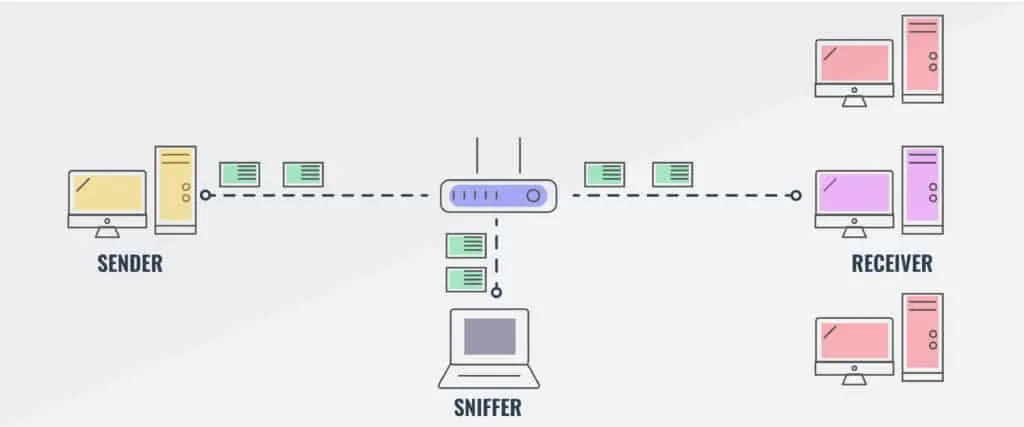
\includegraphics[width=\linewidth]{graphics/networksniffing.png}
    \caption{Een illustratie over network sniffing}
    \label{fig:networksniffing}
\end{figure}

\subsubsection{Netwerkverkeersanalyse toepassen op web scraping}
Bij het bezoeken van een website vindt er een complexe uitwisseling van data plaats tussen de browser van de gebruiker en de server. Deze uitwisseling, die bekend staat als netwerkverkeer, bestaat uit een reeks HTTP-requests en -responses.
Elke HTTP-request wordt door de browser verstuurd en bevat een specifiek verzoek voor een bestand, zoals een JSON-bestand, XML-bestand, HTML-bestand, CSS-stylesheet, JavaScript-bestand of afbeelding. De server ontvangt dit request en genereert een HTTP-response die de gevraagde data bevat. Het proces kan als volgt worden gestructureerd:
\begin{enumerate}
    \item \textbf{Initiatie van een HTTP-request:} Wanneer een gebruiker een URL in de browser invoert of een hyperlink volgt, stuurt de browser een HTTP-request naar de server. Deze request bevat informatie over de gevraagde resource, zoals het type bestand en de locatie ervan op de server.

    \item \textbf{Verwerking door de server:} De server ontvangt de HTTP-request, interpreteert deze en zoekt de gevraagde resource op. Als de resource beschikbaar is, bereidt de server een HTTP-response voor.

    \item \textbf{Terugzending van de HTTP-response:} De server stuurt de HTTP-response terug naar de browser. Deze response bevat de status van de request (bijvoorbeeld 200 OK als het bestand succesvol is gevonden) en de gevraagde data zelf.

    \item \textbf{Rendering door de browser:} De browser ontvangt de HTTP-response en begint met het verwerken en renderen van de ontvangen data. Dit kan het weergeven van een HTML-pagina omvatten, het toepassen van CSS-styling, of het uitvoeren van JavaScript-code om interactieve elementen te creëren.
\end{enumerate}

De JSON-bestanden en XML-bestanden worden gebruikt om gestructureerde data op te slaan en te versturen. Websites maken vaak gebruik van deze bestanden om hun inhoud dynamisch op te bouwen \autocite{DeGroote2022}. Door deze bestanden te analyseren kunnen relevante gegevens worden geïdentificeerd en geëxtraheerd zonder de noodzaak om de complexe HTML-structuur van de webpagina zelf te parsen. Websites maken vaak niet gebruik van de volledige inhoud van deze bestanden. Dit betekent dat deze bestanden meer gegevens bevatten dan zichtbaar is op de website. Dit kan betrekking hebben op extra gegevens, zoals bepaalde producten die niet op de website worden weergegeven. Het kan ook gaan om meer gedetailleerde informatie. Bijvoorbeeld, een bestand kan interne productidentificaties, gedetailleerde specificaties, of voorraadniveaus bevatten die niet direct zichtbaar zijn voor de gebruiker op de website.
\\
\\
Het analyseren van netwerkverkeer kan worden uitgevoerd met tools zoals Wireshark en TCPdump. Deze tools bieden uitgebreide mogelijkheden, maar het gebruik ervan is complex en vereist een diepgaande kennis van beide programma's. Voor een meer toegankelijke benadering kan men gebruik maken van de developer tools in webbrowsers. Deze bevatten een netwerk-tabblad waarop het netwerkverkeer zichtbaar is. Iedere moderne browser beschikt over dergelijke developer tools~\autocite{mdn2023}, waardoor het eenvoudiger is om netwerkverkeer te analyseren zonder de noodzaak van uitgebreide technische kennis. Deze tools kunnen worden gebruikt voor een initiële verkenning van het netwerkverkeer en de website structuur. Voor het automatisch web scrapen wordt gebruik gemaakt van programmeertalen zoals Python, Java en Javascript. Dit onderzoek focust zich enkel op Python.

\section{Webscraping Python-bibliotheken}
In dit hoofdstuk worden alle relevante Python-bibliotheek voor dit onderzoek gedetailleerd beschreven.

\subsection{Requests}
Met 495 miljoen maandelijkse downloads \autocite{Nate2023} is dit de tweede meest gedownloade webscraping Python-bibliotheek.\autocite{Flynn2018}. Deze bibliotheek vereenvoudigt het proces van het verzenden van HTTP-verzoeken en het verwerken van de ontvangen responsen. Requests biedt meerdere pluspunten aan waaronder \autocite{Nate2011}:
\begin{itemize}
    \item \textbf{Beheer van headers}: Headers zijn essentieel voor het simuleren van een menselijke browser en het omzeilen van beveiligingsmaatregelen. De 'requests' bibliotheek biedt de mogelijkheid om aangepaste headers toe te voegen aan verzoeken, waardoor ontwikkelaars meer controle hebben over hoe hun verzoeken worden behandeld door de server.

    \item \textbf{Verwerking van responsen}: Deze bibliotheek stelt ontwikkelaars in staat om de statuscode, headers en de inhoud van een respons te analyseren. Dit is cruciaal voor het valideren van de resultaten van HTTP-verzoeken en voor het implementeren van logica die afhankelijk is van de ontvangen data.

    \item \textbf{Behandeling van cookies}: Cookies spelen een belangrijke rol bij het bijhouden van sessies. De 'requests' bibliotheek biedt tools om cookies te beheren, wat essentieel is voor het behouden van de sessiestatus tussen verschillende verzoeken en het interactief maken van webapplicaties.
\end{itemize}

De 'requests' bibliotheek heeft veel functionaliteiten maar er zijn ook enkele beperkingen waar men rekening mee moet houden:

\begin{itemize}
    \item \textbf{Asynchrone operaties}: De 'requests' bibliotheek ondersteunt geen asynchrone operaties. Dit betekent dat elk verzoek blokkeert totdat een respons is ontvangen, wat kan leiden tot prestatieproblemen in toepassingen die meerdere HTTP-verzoeken tegelijk moeten verwerken.

    \item \textbf{Beperkte ingebouwde foutafhandeling}: Hoewel de 'requests' bibliotheek basale foutafhandeling biedt, kan het nodig zijn om aanvullende mechanismen te implementeren voor complexere foutscenario's, zoals herhaalpogingen bij tijdelijke netwerkfouten of het correct afhandelen van time-outs.

    \item \textbf{Grotere afhankelijkheid van externe bibliotheken}: Voor sommige geavanceerde functionaliteiten, zoals uitgebreide authenticatiemethoden of geavanceerde SSL-configuraties, kan het nodig zijn om aanvullende bibliotheken te gebruiken naast 'requests', wat de complexiteit van de implementatie kan verhogen.
\end{itemize}}

De 'requests' bibliotheek is een krachtige en flexibele tool die de interactie met webservices aanzienlijk vereenvoudigt en verbetert, maar het is belangrijk om bewust te zijn van de beperkingen om ervoor te zorgen dat de gekozen oplossing optimaal aansluit bij de specifieke behoeften van een project.

In codefragment \ref{code:example2} bevinden zich toepassingen van de besproken functionaliteiten van deze Python-bibliotheek.

\begin{lstlisting}[language=python, captionpos=b, caption={Een voorbeeld van de kernfunctionaliteiten van requests.}, label={code:example2}]
    import requests

    # URL om HTTP-requests mee te testen
    url = "https://jsonplaceholder.typicode.com/posts"

    # Aangepaste headers toevoegen aan het verzoek
    headers = {
        "User-Agent": "Mozilla/5.0 (compatible; requests-example/1.0)",
        "Accept": "application/json"
    }

    # Cookies beheren
    cookies = {
        "session_id": "123456"
    }

    try:
        # GET-verzoek verzenden met headers en cookies
        response = requests.get(url, headers=headers, cookies=cookies)

        # Statuscode controleren
        if response.status_code == 200:
            print("Succesvol verzoek!")

        # Headers van de respons weergeven
        print("Response Headers:")
        for header, value in response.headers.items():
            print(f"{header}: {value}")

        # Inhoud van de respons verwerken (aangenomen dat de respons JSON is)
        data = response.json()
        print("\nEerste 5 items in de respons:")
        for item in data[:5]:
            print(item)
        else:
            print(f"Fout bij het verzoek: {response.status_code}")

    except requests.exceptions.RequestException as e:
        print(f"Er is een fout opgetreden: {e}")

    # POST-verzoek verzenden met payload
    payload = {
        "title": "foo",
        "body": "bar",
        "userId": 1
    }

    try:
        post_response = requests.post(url, headers=headers, json=payload, cookies=cookies)

        if post_response.status_code == 201:
            print("\nPOST-verzoek succesvol!")
            print("Response Content:")
            print(post_response.json())
        else:
            print(f"Fout bij het POST-verzoek: {post_response.status_code}")

    except requests.exceptions.RequestException as e:
        print(f"Er is een fout opgetreden bij het POST-verzoek: {e}")

\end{lstlisting}


\subsection{Beautiful Soup 4}
In dit onderdeel wordt dieper ingegaan op het proces van het extraheren van de gewenste data uit deze HTML-code. Hiervoor wordt gebruik gemaakt van de Python-bibliotheek Beautiful Soup 4.
Beautiful Soup is een Python library die speciaal ontworpen is om HTML en XML documenten te parsen. Het biedt een eenvoudige interface om door de structuur van een document te navigeren en specifieke elementen te vinden en te manipuleren. Beautiful Soup 4 heeft een aantal kernfunctionaliteiten \autocite{Soup2004}:

\begin{itemize}
    \item \textbf{Parsen van HTML-code:} Beautiful Soup kan verschillende HTML-parsers gebruiken, zoals 'lxml 'of 'html.parser', om HTML-code om te zetten naar een parseboom. Deze parseboom is een gestructureerde representatie van het document, wat het navigeren vergemakkelijkt.

    \item \textbf{Zoeken naar elementen:} Met behulp van CSS-selectoren of XPath-queries kunnen specifieke elementen in de parseboom worden gevonden. Dit maakt het eenvoudig om bepaalde tags, attributen of inhoud te identificeren en te extraheren.

    \item \textbf{Navigeren van de parseboom:}  De library biedt methoden om door de parseboom te navigeren. Gebruikers kunnen bijvoorbeeld naar de ouder (parent), kinderen (children) of broers en zussen (siblings) van een element gaan. Dit maakt het mogelijk om relaties tussen verschillende elementen in een document te begrijpen en te exploiteren.

    \item \textbf{Manipuleren van elementen:}  Elementen in de parseboom kunnen worden gewijzigd, toegevoegd of verwijderd. Dit biedt flexibiliteit om de structuur en inhoud van een document dynamisch aan te passen.
\end{itemize}

Hoewel Beautiful Soup 4 een krachtige tool is voor webscraping, zijn er enkele beperkingen waarmee rekening moet worden gehouden:

\begin{itemize}
    \item \textbf{Dynamische inhoud:} Beautiful Soup 4 is effectief voor het parsen van statische HTML-pagina's. Echter, voor websites die dynamische inhoud genereren via JavaScript, zoals Single Page Applications, kan Beautiful Soup deze inhoud niet direct parsen. Hiervoor kan men bijvoorbeeld gebruik maken van de Python-bibliotheek Selenium.

    \item \textbf{Complexiteit van de website: } Websites met zeer complexe HTML-structuren, veel geneste elementen en aangepaste tags kunnen moeilijk te parsen zijn, vooral bij gebrek aan duidelijke structuren.
\end{itemize}

Bij het bouwen van een traditionele webscraper  in Python is Beautiful Soup 4 dus een must-have Python-bibliotheek. Het is echter wel belangerijk om de beperkingen van de Python-bibliotheek te begrijpen. In codefragment \ref{code:example3} worden de besproken functionaliteiten toegepast.


\begin{lstlisting}[language=python, captionpos=b, caption=Een voorbeeld van de kernfunctionaliteiten van Beautiful Soup 4, label={code:example3}]
    from bs4 import BeautifulSoup

    # Voorbeeld HTML-content
    html_content = '''
    <!DOCTYPE html>
    <html>
    <head>
        <title>Voorbeeld Pagina</title>
    </head>
    <body>
        <h1>Welkom op mijn website</h1>
        <p class="intro">Dit is een voorbeeldpagina.</p>
        <p class="info">Hieronder staat een lijst met mijn favoriete boeken:</p>
        <ul>
            <li>Python Programming</li>
            <li>Data Science Handbook</li>
            <li>Machine Learning Yearning</li>
        </ul>
        <p class="footer">Contact: example@example.com</p>
    </body>
    </html>
    '''

    # Parseren van HTML
    soup = BeautifulSoup(html_content, 'lxml')

    # Zoeken naar elementen
    title = soup.title.text
    header = soup.h1.text
    intro_paragraph = soup.find('p', class_='intro').text
    items = [li.text for li in soup.find_all('li')]

    # Navigeren door de parseboom
    first_paragraph = soup.body.p.text  # Eerste <p> in <body>
    all_paragraphs = soup.body.find_all('p')

    # Manipuleren van elementen
    new_paragraph = soup.new_tag('p')
    new_paragraph.string = 'Dit is een nieuw alinea toegevoegd door Beautiful Soup.'
    soup.body.append(new_paragraph)

    # Resultaten weergeven
    print("Titel van de pagina:", title)
    print("Header:", header)
    print("Introductieparagraaf:", intro_paragraph)
    print("Boekenlijst:")
    for item in items:
        print(f" - {item}")

    print("Eerste paragraaf in body:", first_paragraph)
    print("Alle paragrafen in body:")
    for p in all_paragraphs:
        print(f" - {p.text}")
\end{lstlisting}

\begin{lstlisting}[caption={De output van code fragment \ref{code:example3}}, label={outuput:example1}]
    Titel van de pagina: Voorbeeld Pagina
    Header: Welkom op mijn website
    Introductieparagraaf: Dit is een voorbeeldpagina.
    Boekenlijst:
     - Python Programming
     - Data Science Handbook
     - Machine Learning Yearning
    Eerste paragraaf in body: Dit is een voorbeeldpagina.
    Alle paragrafen in body:
     - Dit is een voorbeeldpagina.
     - Hieronder staat een lijst met mijn favoriete boeken:
     - Contact: example@example.com
\end{lstlisting}


\subsection{Selenium}
Selenium is een open-source framework voor het automatiseren van webapplicatietests. Het kan echter ook effectief worden gebruikt voor webscraping. Selenium ondersteunt meerdere programmeertalen, waaronder Python, Java, C#, en Ruby. De tool biedt een interface om browsers te besturen, waardoor gebruikers webpagina's kunnen laden, elementen kunnen identificeren en interacties kunnen uitvoeren, zoals klikken en formulierinvoer. De Selenium Python-bibliotheek heeft een aantal kernfunctionaliteiten \autocite{Muthukadan2011}:

\begin{itemize}
    \item \textbf{Multi-browser ondersteuning:} Selenium ondersteunt verschillende browsers, zoals Chrome, Firefox, Safari en Edge. voor ieder van deze browsers zijn er drivers beschikbaar. Deze drivers kunnen gebruikt worden zoals in codefragment \ref{code:example4}. Dit maakt het mogelijk om scraping-taken uit te voeren in een omgeving die lijkt op die van een echte gebruiker.

    \begin{lstlisting}[language=Python, caption={voorbeeld Selenium driver}, captionpos=b, label=code:example4]
        from selenium import webdriver

        driver = webdriver.Firefox()
        driver.get("http://www.python.org")
        driver.close()
    \end{lstlisting}

    \item \textbf{Complexere interacties:} Selenium kan complexe gebruikersinteracties simuleren, zoals het klikken op knoppen, het invullen van formulieren en het navigeren door meerdere pagina's. Dit maakt het mogelijk om gegevens te verzamelen van websites die een bepaalde volgorde van acties vereisen.

    \item \textbf{Rendering van JavaScript:} Veel websites maken gebruik van JavaScript om de gebruikersinterface te renderen. Selenium kan de browser instrueren om de pagina volledig te renderen, waardoor de volledige HTML-structuur beschikbaar komt voor scraping.

\end{itemize}

Ondanks zijn veelzijdigheid heeft Selenium ook enkele beperkingen:

\begin{itemize}
    \item \textbf{Snelheid:} Selenium is doorgaans trager dan andere scraping-methoden. Dit komt doordat het een volledige browser moet opstarten en elke pagina volledig moet laden. Hierdoor kan de verwerkingstijd aanzienlijk toenemen, vooral bij complexe webpagina's.

    \item \textbf{Resource-intensief:} Het uitvoeren van Selenium-scripts vereist veel systeembronnen. Dit is met name problematisch bij het uitvoeren van grote aantallen requests, wat kan leiden tot een verhoogde belasting van CPU en geheugen. Hierdoor kunnen de prestaties van het systeem negatief beïnvloed worden.

    \item \textbf{Browser-afhankelijkheid:} Selenium-scripts zijn afhankelijk van specifieke browserfuncties. Dit betekent dat scripts mogelijk niet uniform werken op alle browsers. Incompatibiliteit tussen verschillende browsers kan leiden tot inconsistent gedrag van de scripts, wat de betrouwbaarheid en robuustheid van de automatisering kan verminderen.
\end{itemize}

Selenium biedt een krachtige set tools voor webscraping via netwerkverkeersanalyse, met name wanneer het gaat om dynamische en interactieve webpagina's. Hoewel het enkele beperkingen heeft, zoals prestatie- en onderhoudsproblemen, maakt de flexibiliteit en de mogelijkheid om realistische gebruikersinteracties te simuleren het een waardevolle tool voor specifieke scraping-taken. In de context van deze thesis zal Selenium worden gebruikt om de mogelijkheden en uitdagingen van webscraping via netwerkverkeersanalyse verder te onderzoeken.

\section{Anti webscraping maatregelen}
Webscraping, het geautomatiseerd verzamelen van gegevens van websites, heeft de laatste jaren aanzienlijke aandacht gekregen. Deze techniek biedt talloze voordelen, zoals het verzamelen van gegevens voor marktanalyse, prijsvergelijking en wetenschappelijk onderzoek. Echter, webscraping kan ook nadelige gevolgen hebben voor website-eigenaren, waaronder verhoogde serverbelasting, schending van gebruiksvoorwaarden en potentiële inbreuken op auteursrechten en privacywetten. Om deze redenen nemen steeds meer organisaties maatregelen om webscraping te detecteren en te voorkomen.

\subsection{Detectie van webscraping}
Detectie van webscraping speelt een belangrijke rol bij het beheren en controleren van geautomatiseerde dataverzameling op websites. Webscraping wordt doorgaans gedetecteerd door het analyseren van webverkeerspatronen en gebruikersgedrag dat afwijkt van de norm. De kenmerkende aspecten van webscraping omvatten, maar zijn niet beperkt tot, een hoog volume aan dataverzoeken binnen een kort tijdsbestek, het systematisch ophalen van gegevens van specifieke webpagina's, en patronen in het aanvragen van informatie die consistent zijn over meerdere sessies. Verder kunnen scrapers pogingen doen om detectie te vermijden door het imiteren van menselijk gedrag, zoals het willekeurig variëren van de tijd tussen verzoeken of het gebruiken van verschillende IP-adressen.
Deze basisprincipes vormen het fundament voor meer gespecialiseerde detectietechnieken en -strategieën die verderop in dit hoofdstuk worden besproken. Door een grondig begrip van deze principes kunnen ontwikkelaars en cybersecurity professionals effectievere maatregelen ontwerpen om webscraping te identificeren en tegen te gaan.

\subsubsection{Signature-based Detectie}
Signature-based~\autocite{Vastel2023} detectie is een traditionele benadering waarbij specifieke kenmerken van webscrapingverkeer worden geïdentificeerd. Deze kenmerken kunnen onder andere bestaan uit:
\begin{itemize}
    \item \textbf{Unieke user-agents: } Scrapers maken vaak gebruik van specifieke user-agents om zich te identificeren. Door deze user-agents te monitoren, kunnen websites verdachte activiteiten detecteren.

    \item \textbf{Ongebruikelijke request headers: }Scrapers kunnen afwijkende request headers bevatten die wijzen op automatische verwerking in plaats van menselijke interactie.

    \item \textbf{Hoge frequentie van requests: }Scrapers maken vaak een groot aantal requests in een korte tijdspanne, wat een afwijkend patroon kan vormen ten opzichte van normaal gebruikersgedrag.
\end{itemize}

Deze methode is relatief eenvoudig te omzeilen door scrapers die hun sporen proberen te verbergen. Door bijvoorbeeld willekeurige user-agents te gebruiken of de frequentie van requests aan te passen, kunnen scrapers de detectie ontwijken.

\subsubsection{Gedragsgebaseerde Detectie}
Behavioral-based detectie gaat een stap verder door het gedrag van gebruikers te analyseren en afwijkingen ~\autocite{Lotfi2021} te identificeren. Deze methode maakt vaak gebruik van machine learning en deep learning algoritmes om complexe patronen in het netwerkverkeer te herkennen. Enkele veelgebruikte technieken zijn:
\begin{itemize}
    \item \textbf{Anomaliedetectie: } Door het identificeren van afwijkingen van normaal gebruikersgedrag kunnen webscraping activiteiten worden gedetecteerd.
    \item \textbf{Clustering: }Vergelijkbare request patronen kunnen worden geclusterd om verdachte groepen te identificeren.
\end{itemize}


\subsection{Preventie van webscraping}
Naast detectie is preventie essentieel om webscraping te ontmoedigen en te stoppen. Preventieve maatregelen kunnen zowel passieve als actieve benaderingen omvatten. Passieve methoden, zoals het gebruik van robots.txt-bestanden en anti-scraping headers, geven richtlijnen aan legitieme bots over welke delen van de website toegankelijk zijn. Actieve methoden zijn onder meer het blokkeren van verdachte IP-adressen, het gebruik van dynamische inhoudsgeneratie en de implementatie van JavaScript-obfuscatie. Door deze technieken te combineren, kunnen websites hun gegevens beter beschermen tegen ongeautoriseerde toegang en extractie.

\subsubsection{Passieve technieken}
Passieve technieken zijn ontworpen om webscrapers te identificeren en af te schrikken zonder hen actief te blokkeren. Deze methoden richten zich op het herkennen van niet-menselijke interacties met webpagina's en kunnen waardevolle inzichten geven in verdachte activiteiten. Enkele veelgebruikte methoden zijn:

\begin{itemize}
    \item \textbf{CAPTCHAs: } Dit staat voor 'completely automated public Turing test to tell computers and humans apart'. Deze  test, bestaande uit letters, cijfers of afbeeldingen, is bedoeld om te verifiëren dat de aanvraag van een mens komt en niet van een bot. CAPTCHAs worden vaak gebruikt bij het invullen van formulieren of bij het aanvragen van gevoelige informatie.

    \item \textbf{Honey Pots:} Dit zijn verborgen elementen op een webpagina die alleen zichtbaar zijn voor bots. Wanneer een bot met deze elementen interageert, wordt dit als een sterke indicator gezien dat het om een bot gaat. Deze techniek helpt bij het identificeren van geautomatiseerde aanvallen zonder de gebruikerservaring te verstoren.
\end{itemize}

\subsubsection{Actieve technieken}
Actieve technieken richten zich op het actief blokkeren van webscrapers. Deze methoden zijn bedoeld om de toegang van bots tot webpagina's en gegevens effectief te beperken of volledig te voorkomen. Enkele voorbeelden zijn:

\begin{itemize}
    \item \textbf{Rate Limiting:} Door het aantal aanvragen dat een IP-adres of gebruiker in een bepaalde tijd kan doen te beperken, wordt het voor bots moeilijker om grote hoeveelheden data te verzamelen. Deze techniek helpt bij het behouden van de prestaties van de website en beschermt tegen overmatige dataverzoeken.
    \item \textbf{IP-banning:} Verdachte IP-adressen kunnen geblokkeerd worden om verdere aanvallen te voorkomen. Deze methode is effectief tegen bekende IP-adressen, maar vereist voortdurende monitoring en updates van de lijst met geblokkeerde adressen.
\end{itemize}

\section{Ethische aspecten}
Webscraping, het proces waarbij geautomatiseerde scripts of programma's gegevens van websites verzamelen, biedt enorme mogelijkheden voor data-analyse. Echter, het brengt ook diverse ethische uitdagingen met zich mee die aandacht vereisen. In dit hoofdstuk worden de belangrijkste ethische kwesties in verband met webscraping besproken, waaronder privacy, intellectuele eigendom en misbruik. Verder worden ethische richtlijnen en best practices besproken om verantwoord gebruik van webscraping te waarborgen.

\subsection{Privacy}
\subsubsection{Inbreuk op de privacy van gebruikers}
Webscraping kan leiden tot het verzamelen van persoonlijke gegevens zonder expliciete toestemming van de gebruiker, vooral wanneer netwerkverkeersanalyse wordt toegepast. Dit kan ernstige privacy-inbreuken veroorzaken, waarbij gevoelige informatie zoals naam, adres en andere persoonlijke details zonder toestemming worden vastgelegd en mogelijk misbruikt.

\subsubsection{Gegevensbeschermingswetgeving}
Wetgevingen zoals de Algemene Verordening Gegevensbescherming (AVG) in de EU en de California Consumer Privacy Act (CCPA) in de VS stellen strikte eisen aan de verzameling en verwerking van persoonlijke gegevens. Deze wetgevingen zijn ook van toepassing op webscraping en vereisen dat organisaties transparant zijn over welke gegevens zij verzamelen, hoe deze worden gebruikt en dat zij toestemming van de gebruikers verkrijgen.

\subsubsection{Anoniemisering en pseudonimisering}
Om de privacy te beschermen, kunnen technieken zoals anonimisering en pseudonimisering worden toegepast. Anonimisering verwijdert alle identificeerbare informatie uit de dataset, terwijl pseudonimisering de identificeerbare informatie vervangt door een pseudoniem. Hoewel deze technieken de privacy verbeteren, zijn ze niet zonder beperkingen, omdat geavanceerde methoden soms nog steeds kunnen leiden tot heridentificatie van individuen.

\subsection{Intellectueel Eigendom}
\subsubsection{Copyright en auteursrecht}
Het kopiëren en hergebruiken van data van websites roept juridische vragen op met betrekking tot auteursrecht. De originele content op websites kan auteursrechtelijk beschermd zijn, en het ongeoorloofd kopiëren ervan kan leiden tot juridische geschillen en sancties.

\subsubsection{Terms of Service}
Websites hanteren vaak Terms of Service (ToS) die expliciet regels en beperkingen vastleggen omtrent webscraping. Het niet naleven van deze voorwaarden kan juridische gevolgen hebben, zoals toegang tot de website verliezen of juridische claims van de website-eigenaar.

\subsubsection{Databasebescherming}
Naast auteursrecht kunnen databases specifieke juridische bescherming genieten onder wetten zoals de Europese Databankenrichtlijn. Webscraping kan inbreuk plegen op deze bescherming, vooral wanneer het systematisch en op grote schaal gebeurt.

\subsection{Systeembelasting}
\subsubsection{Overbelasting van servers}
Overmatige webscraping kan leiden tot prestatieproblemen voor websites en servers, wat de gebruikerservaring kan verslechteren en extra kosten kan veroorzaken voor website-eigenaren.

\subsubsection{Denial-of-service aanvallen}
In extreme gevallen kan webscraping worden gebruikt om Distributed Denial of Service (DDoS)-aanvallen uit te voeren, waardoor websites onbereikbaar worden en aanzienlijke schade kunnen ondervinden.

\subsection{Best practices}
\subsubsection{Transparantie}
Het is cruciaal dat organisaties transparant zijn over hun webscraping-activiteiten en de doelen die zij daarmee nastreven. Dit helpt bij het opbouwen van vertrouwen en het waarborgen van ethische standaarden.

\subsubsection{Minimale gegevensverzameling}
Webscraping moet zo worden uitgevoerd dat de privacy van gebruikers minimaal wordt aangetast. Dit houdt in dat alleen de noodzakelijke gegevens worden verzameld en dat er maatregelen worden genomen om de impact op privacy te minimaliseren.

\subsubsection{Ethische codes}
Er zijn bestaande ethische codes voor onderzoekers en ontwikkelaars~\autocite{Don2018} die richtlijnen bieden voor verantwoord gebruik van webscraping. Deze codes benadrukken het belang van eerlijkheid, transparantie en respect voor privacy en intellectueel eigendom.
\\
\\
De belangrijkste ethische uitdagingen van webscraping omvatten privacy-inbreuken, juridische kwesties in verband met intellectueel eigendom, het potentiële misbruik van gegevens en de impact op systeemprestaties. Het naleven van ethische richtlijnen en best practices is cruciaal om verantwoord webscraping te waarborgen.